\chapter{Implementazione della procedura}\label{second-c}
Come descritto nel precedente capitolo, la procedura di decisione per problemi
appartenenti al frammento \emph{guarded} è formata da una fase di \emph{preprocessing} e 
una fase di risoluzione tramite $\prec$-\emph{ordered resolution} e \emph{factorization}. 
\begin{figure}[H]
    \incfig{architettura-2}
    \caption{Struttura di \textsc{Vampire} prima delle modifiche}
\end{figure}
L'idea per l'implementazione della procedura è:
\begin{enumerate}
    \item costruire un nuovo \emph{preprocessor} che trasformi le formule \emph{guarded} in clausole e sostituirlo nel sistema
    \item implementare una nuova inferenza ($\prec$\emph{-ordered resolution}) e ``iniettarla" nell'algoritmo di saturazione
    \item eliminare tutte le inferenze non necessarie dall'algoritmo di saturazione 
\end{enumerate}
\begin{figure}[H]
    \incfig{architettura-3}
    \caption{Struttura di \textsc{Vampire} dopo le modifiche}
\end{figure}
\section{Preprocessing}
Per quanto riguarda la fase di \emph{preprocessing}, è stato sviluppato un \emph{preprocessor} per trattare problemi 
appartenenti al frammento \emph{guarded}. Questa componente è stata implementata seguendo l'architettura 
del \emph{preprocessor} predefinito di \textsc{Vampire}.
\begin{algorithm}
    \caption{Preprocessing}
    \begin{algorithmic}
        \State \textbf{var} problem : sets of guarded formula
        \State \textbf{var} result : sets of guarded clause 
        \State problem = \emph{NNF}(problem)
        \State problem = \emph{flatten}(problem)
        \State problem =$\text{\emph{Struct}}_\forall$(problem)
        \State problem = \emph{skolemize}(problem)
        \State result = \emph{clausify}(problem)
        \State \emph{computeVarDepth}(result)
        \State \underline{\textbf{return} result}
    \end{algorithmic}
\end{algorithm}

\emph{NNF, flatten, skolemize} e \emph{clausify} (descritte in \ref{sec-prepro}) sono le funzioni di 
\textsc{Vampire} che vengono sfruttate per la trasformazione del problema.
Invece le funzioni $\text{\emph{Struct}}_\forall$ e \emph{computeVarDepth} vengono implementate ex-novo in quanto non presenti 
nel sistema. 

$\text{\emph{Struct}}_\forall$ è una funzione ricorsiva che sfrutta la struttura ad albero delle formule.
\begin{figure}[H]
    \incfig{tree}
    \caption{Struttura ad albero della formula}
\end{figure}
L'intero albero sintattico della formula viene visitato tramite una visita post-order. Durante la visita, l'algoritmo 
controlla se nell'intero albero sono presenti formule del tipo $\forall \bar{x}(a \lor A)$ con almeno una variabile libera.
Nel caso venga trovata una formula in questa forma, viene applicata la trasformazione strutturale 
$\text{\emph{Struct}}_\forall$.

\begin{algorithm}[H]
    \caption{Visita post-order}
    \begin{algorithmic}
        \Function{\textsc{PostOrderVisit}}{input : formula}
            \Case{connective \textbf{of} input}
                \Switch{$\top,\bot$, Literal}
                    \State \underline{\textbf{return} input}
                \EndSwitch
                \Switch{$\lnot,\exists$}
                    \State \underline{\textbf{return} \textsc{PostOrderVisit}(subformula \textbf{of} input)}
                \EndSwitch
                \Switch{$\rightarrow,\leftrightarrow$}
                    \State \textbf{var} left, right : formula
                    \State left = \textsc{PostOrderVisit}(left subformula \textbf{of} input)
                    \State right = \textsc{PostOrderVisit}(right subformula \textbf{of} input) 
                    \State \underline{\textbf{return} input}
                \EndSwitch
                \Switch{$\land,\lor$}
                    \ForAll{subformula \textbf{in} input}
                        \State subformula = \textsc{PostOrderVisit}(subformula)
                    \EndFor
                    \State \underline{\textbf{return} input} 
                \EndSwitch
                \Switch{$\forall$}
                    \State \textbf{var} subformula : formula
                    \State subformula = \textsc{PostOrderVisit}(subformula \textbf{of} input)
                    \If{(connective \textbf{of} subformula \textbf{is} $\lor$) $\land$ (\emph{hasFreeVar}(input))}
                        \State  input=$\text{\emph{Struct}}_\forall$(input)
                    \EndIf
                    \State \underline{\textbf{return} input}
                \EndSwitch  
            \EndCase
        \EndFunction
    \end{algorithmic}
\end{algorithm}
Per l'implementazione della trasformazione strutturale, si segue la definizione \ref{struct-def}.
\begin{algorithm}[H]
    \caption{$\text{\emph{Struct}}_\forall$}
    \begin{algorithmic}
        \Function{\textsc{$\text{\emph{Struct}}_\forall$}}{input : formula}
        \State \textbf{var} new, $\alpha$ : formula
        \State \textbf{var} $\bar{y}$ : sets of free variables 
        \State $\bar{y} =$ \emph{saveFreeVariable}(input)
        \State $\alpha =$ \emph{createNewLiteral}($\bar{y}$)
        \State new = \emph{generateNewFormula}($alpha$,input)
        \State \emph{addFormulaToUnits}(new)
        \State input = $\alpha$
        \State \underline{\textbf{return} input}
        \EndFunction
    \end{algorithmic}
\end{algorithm}
In primis viene creato un nuovo letterale/formula atomica $\alpha$ con le variabili libere $\bar{y}$
tramite la funzione \emph{createNewLiteral}() e, subito dopo, la formula in input viene sostituita da $\alpha$. Successivamente 
viene generata una nuova formula del tipo $\forall\bar{x}\bar{y}(\lnot a \lor \lnot\alpha \lor A)$ tramite la 
funzione \emph{generateNewFormula}() e viene aggiunta al problema con la funzione 
\emph{addFormulaToUnits}().

La funzione \emph{computeVarDepth}() calcola il parametro \emph{VarDepth} (definizione \ref{var-def}) di ogni letterale 
presente nelle clausole risultanti. Per salvare il risultato è stata modificata la classe \verb|Literal| ed è stato aggiunto un attributo 
privato \emph{$varDepth$}. 
La visita dei termini per il calcolo della \emph{VarDepth} è stato semplificato grazie a un iteratore 
già implementato in \textsc{Vampire}. \emph{computeVarDepth}() è diviso in due componenti:
\begin{enumerate}
    \item la prima funzione scorre i termini più esterni del letterale (termini rossi nella figura \ref{fig:lit-it}) tramite un \verb|SubtermIterator|
    \item la seconda funzione va in profondità e scorre i sottotermini (termini verdi nella figura \ref{fig:lit-it}) tramite un altro \verb|SubtermIterator|
\end{enumerate}
\begin{figure}[H]
    \centering
    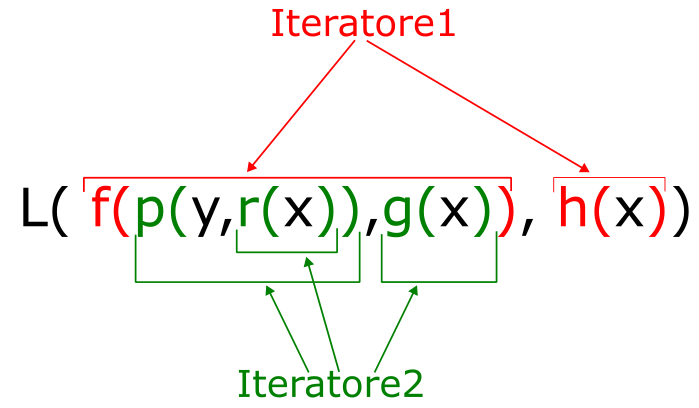
\includegraphics[width=\columnwidth]{figures/literal-iterator.png}
    \caption{Uso degli iteratori per il calcolo della \emph{VarDepth}}
    \label{fig:lit-it}
\end{figure}
In questo caso la prima funzione è iterativa, mentre la seconda è ricorsiva per sfruttare la struttura del letterale.
\begin{algorithm}[H]
    \caption{Prima funzione che scorre i termini esterni del letterale}
    \begin{algorithmic}
        \Function{\textsc{ComputeVarDepth1}}{lit : literal}
        \If{literal \textbf{is} ground}
            \State setLiteralVarDepth(-1, lit)
            \State \underline{\textbf{return}}
        \EndIf
        \State \textbf{var} max, varDepth : int
        \State max = 0
        \ForAll{term \textbf{in} lit} \Comment{Iteratore1 qui scorre i termini esterni}
            \State varDepth = 0
            \State varDepth = 1 + \textsc{ComputeVarDepth2}(term)
            \If{max $<$ varDepth}
                \State max = varDepth
            \EndIf
        \EndFor
        \State setLiteralVarDepth(max, lit)
        \EndFunction
    \end{algorithmic}
\end{algorithm}
Se il letterale è \emph{ground}\footnote{Un letterale è detto \emph{ground} se è privo di variabili}, la \emph{VarDepth} di \emph{lit} viene impostata a $-1$ tramite la funzione 
\emph{setLiteralVarDepth()}.
Nel caso non sia \emph{ground}, allora viene calcolata la massima profondità di ciascun termine esterno tramite la seconda funzione \textsc{ComputeVarDepth2}().
Alla fine il risultato sarà la massima profondità calcolata tra tutti i termini. 
\begin{algorithm}[H]
    \caption{Seconda funzione che scorre i sottotermini in profondità}
    \begin{algorithmic}
        \Function{\textsc{ComputeVarDepth1}}{term : term of literal}
        \State \textbf{var} max, varDepth : int
        \State max = 0
        \ForAll{subterm \textbf{in} term} \Comment{Iteratore2 qui scorre i sottotermini}
            \State varDepth = 0
            \State varDepth = 1 + \textsc{ComputeVarDepth2}(subterm) \Comment{Visita in profondità}
            \If{max $<$ varDepth}
                \State max = varDepth
            \EndIf
        \EndFor
        \State \underline{\textbf{return} max}
        \EndFunction
    \end{algorithmic}
\end{algorithm}
\section{Resolution}
La nuova inferenza implementata, denominata $\prec$-\emph{ordered resolution}, eredita la classe \\\verb|GeneratingInferenceEngine| (figura \ref{fig:genengineclass}), 
 in modo da avere a disposizione tutti i metodi necessari per essere inserita 
nell'algoritmo di saturazione e generare nuove clausole.
La funzione principale di questa classe è \emph{generateClause}() che sfrutta le varie strutture 
dati messe a disposizione da \textsc{Vampire}. 

Il metodo viene eseguito dopo la selezione di una clausola e la conseguente attivazione. La struttura dati fondamentale 
è l'indice che tiene traccia di tutte le clausole e permette di trovarne una da unificare con quella selezionata.
Sia $\{A_1\}\cup R_1$ clausola selezionata, allora il risultato della query sull'indice viene salvato 
in un altra struttura dati che comprende:
\begin{itemize}
    \item una clausola $\{\lnot A_2\}\cup R_2$ candidata a unificare con la clausola selezionata 
    \item un letterale $\{\lnot A_2\}$ candidato all'unificazione con uno dei letterali della clausola selezionata (in questo caso $\{A_1\}$)
\end{itemize} 
\begin{algorithm}[H]
    \caption{Funzione \emph{generateClause}()}
    \begin{algorithmic}
        \State \textbf{var} selectedLiteral, candidateLiteral : literal
        \State \textbf{var} selectedClause, candidateClause, result : clause
        \If{\textsc{IsMaximal}(selectedLiteral, selectedClause) $\land$ \textsc{IsMaximal}(candidateLiteral)}
            \State result = \emph{unify(selectedClause, candidateClause)}
            \State \underline{\textbf{return} result}
        \Else
            \State \underline{\textbf{return} NULL}
        \EndIf
    \end{algorithmic}
\end{algorithm}
Sia $\prec$ un ordinamento definito come prescritto dalla definizione \ref{ord-def}.
La funzione \emph{generateClause}() verifica se il letterale 
$\{A_1\}$ in $\{A_1\}\cup R_1$ e il letterale $\{\lnot A_2\}$ in $\{\lnot A_2\}\cup R_2$ sono massimali 
(secondo l'ordinamento $\prec$) tramite la funzione \textsc{IsMaximal}() .
Nel caso siano massimali, allora viene applicata la \emph{resolution} e l'unificazione tramite la funzione \emph{unify}().
\begin{equation*}
    \begin{gathered}
        \underline{\{\underline{A_1}\} \lor R_1 \quad\{\underline{\lnot A_2}\}\lor R_2}\\
        (R_1 \lor R_2)\theta
    \end{gathered}
\end{equation*}
In caso contrario non viene generata alcuna clausola.
\begin{algorithm}[H]
    \caption{Funzione che controlla se un letterale è il massimale in una clausola}
    \begin{algorithmic}
        \Function{\textsc{IsMaximal}}{maxLit : literal, cl : clause}
            \ForAll{lit \textbf{in} cl}
                \State varDepth = \emph{getVarDepth}(lit)
                \If{(max$<$varDepth) $\land$ (\emph{Var}(lit)$\not\subseteq$\emph{Var}(maxLit))}
                    \State \underline{\textbf{return} $\bot$}
                \EndIf
            \EndFor
            \State \underline{\textbf{return} $\top$}
        \EndFunction
    \end{algorithmic}
\end{algorithm}
Seguendo la definizione \ref{ord-def}, la funzione \textsc{IsMaximal}() controlla se 
un letterale \emph{maxLit} è massimale nella clausola ovvero:
\begin{itemize}
    \item se la \emph{VarDepth} di \emph{maxLit} è maggiore o uguale di tutte le \emph{VarDepth} degli altri letterali nella clausola, o
    \item se l'insieme delle variabili di \emph{maxLit} contiene l'insieme delle variabili degli altri letterali nella clausola
\end{itemize}
La funzione restituisce $\bot$ se entrambe le condizioni non sono rispettate.
\section{Classificazione}\label{class}
A fini sperimentali, viene implementato un classificatore per riconoscere, tra un insieme di problemi casuali,
quali di questi appartengono al frammento \emph{guarded}.
Il classificatore viene richiamato dopo il \emph{parser} di \textsc{Vampire} 
ed è composto da due funzioni principali; una per analizzare le formule arbitrarie della logica del primo ordine e un'altra per analizzare clausole.

La prima funzione sfrutta, come il \emph{preprocessor}, 
la struttura ad albero della formula ed è dunque ricorsiva.
\begin{algorithm}[H]
    \caption{Visita dell'albero della formula parte 1}
    \begin{algorithmic}[1]
        \Function{\textsc{Visit}}{input : formula}
            \Case{connective \textbf{of} input}
                \Switch{$\top,\bot$, Literal}
                    \State \underline{\textbf{return} $\top$}
                \EndSwitch
                \Switch{$\lnot$}
                    \State \underline{\textbf{return} \textsc{Visit}(subformula \textbf{of} input)}
                \EndSwitch
                \Switch{$\rightarrow,\leftrightarrow$}
                    \State \textbf{var} left, right : formula
                    \State left = \textsc{Visit}(left subformula \textbf{of} input)
                    \If{left $=\top$}
                        \State \underline{\textbf{return} \textsc{Visit}(right subformula \textbf{of} input)}
                    \EndIf
                    \State \underline{\textbf{return} $\bot$}
                \EndSwitch
                \Switch{$\land,\lor$}
                    \ForAll{subformula \textbf{in} input}
                        \State subformula = \textsc{Visit}(subformula)
                        \If{subformula $\neq \top$}
                            \State \underline{\textbf{return} $\bot$}
                        \EndIf
                    \EndFor
                    \State \underline{\textbf{return} $\top$} 
                \EndSwitch
                \Switch{$\exists$}
                    \State \textbf{var} subformula : formula
                    \State \textbf{var} vars : sets of bounded variables 
                    \State \textbf{var} lit : literal
                    \State \textbf{var} guardFound : bool
                    \State subformula = subformula \textbf{of} input
                    \State vars = \emph{getBoundedVariables}(input)
                    \If{connective \textbf{of} subformula \textbf{is} $\land$} \label{exists}
                        \State guardFound $=\bot$
                        \While{sub-subformula \textbf{in} subformula $\land$ guardFound $=\bot$}
                            \If{sub-subformula \textbf{is} Literal}
                                \State lit = literal \textbf{of} sub-subformula
                                \If{\emph{isPositive}(lit) $\land$ \emph{isGuard}(lit, vars)} \label{pos-guard}
                                    \State guardFound = $\top$
                                \EndIf
                            \EndIf
                        \EndWhile
                        \If{guardFound $==\top$}
                            \State \underline{\textbf{return} \textsc{Visit}(subformula)} 
                        \Else
                            \State \underline{\textbf{return} $\bot$}
                        \EndIf
                    \Else 
                        \State \underline{\textbf{return} $\bot$}
                    \EndIf
                \EndSwitch
                \algstore{myalg} 
            %\EndCase
        %\EndFunction
    \end{algorithmic}
\end{algorithm}

\begin{algorithm}[H]
    \caption{Visita dell'albero della formula parte 2}
    \begin{algorithmic}[1]
        \algrestore{myalg}
            \Switch{$\forall$}
                \State \textbf{var} subformula : formula
                \State \textbf{var} vars : sets of bounded variables 
                \State \textbf{var} lit : literal
                \State \textbf{var} guardFound : bool
                \State subformula = \emph{getSubformula}(input)
                \State vars = \emph{getBoundedVariables}(input)
                \State left = \emph{getLeft}(subformula)
                \If{(connective \textbf{of} subformula \textbf{is} $\rightarrow$) $\land$ (left \textbf{is} Literal)} \label{forall-imp}
                    \State lit = literal \textbf{of} left
                    \If{\emph{isPositive}(lit) $\land$ \emph{isGuard}(lit, vars)} \label{pos-guard-for}
                        \State \underline{\textbf{return} \textsc{Visit}(right subformula \textbf{of} subformula)} 
                    \Else
                        \State \underline{\textbf{return} $\bot$}
                    \EndIf
                \ElsIf{connective \textbf{of} subformula \textbf{is} $\lor$} \label{forall-or}
                    \State guardFound = $\bot$
                    \While{subformula \textbf{in} input $\land$ guardFound $=\bot$}
                        \If{subformula \textbf{is} Literal}
                            \State lit = literal \textbf{of} subformula
                            \If{\emph{isNegative}(lit) $\land$ \emph{isGuard}(lit, vars)} \label{neg-guard}
                                \State guardFound = $\top$
                            \EndIf
                        \EndIf
                    \EndWhile
                    \If{guardFound $=\top$}
                        \State \underline{\textbf{return} \textsc{Visit}(subformula)} 
                    \Else
                        \State \underline{\textbf{return} $\bot$}
                    \EndIf
                \EndIf
                \State \underline{\textbf{return} $\bot$}
            \EndSwitch 
        \EndCase
        \EndFunction
    \end{algorithmic}
\end{algorithm}
Durante la visita l'algoritmo controlla se nell'intero albero sono presenti formule del tipo: 
\begin{itemize}
    \item $\forall\bar{x}(a \rightarrow A)$ (riga \ref{forall-imp}), 
    \item $\forall\bar{x}(a \lor A)$ (riga \ref{forall-or}),
    \item $\exists\bar{x}(a \land A)$ (riga \ref{exists})
\end{itemize}
Nel primo caso verifica che $a$ sia un letterale positivo e una guardia tramite
 le funzioni \emph{isPositive}() e \emph{isGuard}() (riga \ref{pos-guard-for}). 
Nel secondo e nell'ultimo caso si scorrono tutte le sottoformule per trovare, rispettivamente, 
una guardia negativa (riga \ref{neg-guard}) e una guardia positiva (riga \ref{pos-guard}).
\begin{algorithm}
    \caption{Funzione che verifica se un letterale è una guardia}
    \begin{algorithmic}
        \Function{\textsc{IsGuard}}{lit : literal, vars : sets of variables}
            \State \textbf{var} literalVars : sets of variables
            \State literalVars = getVariablesOf(lit)
            \ForAll{variable \textbf{in} vars}
                \State \textbf{var} foundVariable = $\bot$
                \While{litVar \textbf{in} literalVars $\land$ foundVariable $==\bot$}
                    \If{litVar $==$ variable}
                        \State foundVariable = $\top$
                    \EndIf
                \EndWhile
                \If{foundVariable $==\bot$}
                    \State \underline{\textbf{return} $\bot$}
                \EndIf
            \EndFor
            \State \underline{\textbf{return} $\top$}
        \EndFunction
    \end{algorithmic}
\end{algorithm}

La funzione \textsc{IsGuard}() verifica se un letterale è una guardia, ovvero se contiene 
almeno una volta le variabili libere \emph{vars} delle altre sottoformule. 

\begin{algorithm}[H]
    \caption{Funzione che verifica se una clausola è \emph{guarded}}
    \begin{algorithmic}
        \State \textbf{var} cl : clause
        \State \textbf{var} vars : clause variables set
        \State \textbf{var} checkGuard : bool
        \State checkGuard = $\bot$
        \ForAll{lit \textbf{in} cl}
            \If{\emph{isNegative(lit)} $\land$ foundVariable $==\bot$}\label{cl-guard-neg}
                \State checkGuard = \textsc{IsGuard}(lit, vars)
                \If{checkGuard $==\top$}
                    \State \textbf{continue}
                \EndIf
            \EndIf
            \ForAll{term \textbf{in} lit} \label{term-1}
                \If{$\lnot$\emph{containsAllVariablesOfClause}(term,vars)} \label{term-2}
                    \State \underline{\textbf{return} $\bot$}
                \EndIf
            \EndFor
        \EndFor
        \State \underline{\textbf{return} checkGuard}
    \end{algorithmic}
\end{algorithm}
La seconda funzione che analizza le clausole verifica se esiste una guardia negativa (riga \ref{cl-guard-neg}), 
tramite la funzione \textsc{IsGuard}(), e se i termini funzionali non ground contengono 
tutte le variabili della clausola (righe \ref{term-1}, \ref{term-2}).



